\documentclass[12pt]{article}
\usepackage[top=1in, bottom=1in, left=1in, right=1in]{geometry}
\usepackage{setspace}
\usepackage{amsmath,amsthm}
\usepackage{amssymb}
\usepackage{cite}
\renewcommand{\rmdefault}{bch} % change default font
\usepackage[english]{babel}
\usepackage[utf8]{inputenc}
\usepackage{tikz} 
\usetikzlibrary{arrows,decorations.pathmorphing,backgrounds,fit,positioning,shapes.symbols,chains}
\newtheorem{condition}{Condition}
%%%%%%%%%%%%%%%%
\usepackage{booktabs} %table
%%%%%%%%%%%%%%%%
\begin{document}
\title{Research Proposal}
\author{Qin Kan}
\date{\today}
\maketitle
\begin{spacing}{1.5}
%\section{ABSTRACT}
%I am a Senior Project Manager at Shanghai Electric(a chinses multinational power generation and electrical equipment manufacturing company) with an interest in contributing to a deeper understanding of loyalt programs (LPs). LPs are prevalent across a wide range of industries and have enjoyed an increase in membership participation (Berry 2013)\cite{berry2013bulking}.Especially, I employ field, if LPs have a wide range of applications, the company can potentially gain more repeat businesses, at the same time, gather detailed consumer insights that allow them to deliver targeted marketing activities (Ailawadi et al. 2010; Liu 2007)\cite{ailawadi2010empirical}\cite{liu2007long}.
\section{Introduction}
 Loyalt programs (LPs), designed to maintain and enhance the strength of the customer-firm relationship, as important customer relationship management systems (Kopalle et al. 2012; Liu 2007; Bijmolt et al. 2011)\cite{kopalle2012joint}\cite{liu2007long}\cite{bijmolt2011loyalty}. LPs have increased in popularity, and have been studied extensively in the academic literature, I have preliminary combed the relevant literature. 

 Nowadays, various firms have initiated LPs, which have applied across a wide range of industies, including retail, airlines, hospitality, and financial services. These firms have enjoyed an increase in membership participation (Berry 2013)\cite{berry2013bulking}, just as the CEO of Starbucks, Kevin Johnson said during the company’s first-quarter earnings call in 2019. "The number of rewards members increased 14 percent from the first quarter a year earlier. The decade-old program counts more than 16.3 million people as active members, who account for about 40 percent of Starbucks’ transactions."

 Because, the firms can potentially gain more repeat businesses and, at the same time, gather detailed consumer insights that allow them to deliver targeted marketing activities (Ailawadi et al. 2010; Liu 2007)\cite{ailawadi2010empirical}\cite{liu2007long}. While most loyalty programs give away a free product after a certain number of purchases, many companies use their programs as marketing tools and vehicles for collecting customer behavioral data (Robbie Kellman Baxter 2015)\cite{baxter2015membership}. Starbucks expanded its loyalty program to resemblea membership organization,there are three tiers, welcome level member, green member, and gold member. Users who register their rechargeable gift cards online gain access to discounts and customized offers, and they get to try new products first. 

 Just like the following pictures show, the Starbucks has launched a lot of rewards and membership benefits, such as, birthday drink, discount off drink or meal, anniversary drink coupon, taste of gold free drink coupon, and so on. But, which is the more effective reward and benefit for the different level members?  
 
%how to distinguish these rewards and benefits in essence? And, 

 \begin{figure}[ht]
\centering
\includegraphics[scale=0.1265]{picture/rewards.jpeg}
\qquad
\includegraphics[scale=0.11]{picture/member.jpeg}
\caption{Starbucks rewards and benefits (from Starbucks' App)}
\label{fig:label}
\end{figure}
% I employ field, the electrical equipment manufacturing industry, preparing to apply LPs on a large scale.
%If implemented,  Therefore, I decided to study LPs with an interest in contributing to a deeper understanding of LPs, and put into use more areas.

\subsection{Summary of findings}
The insights from my study can be classified into three categories: effect of rewards, effect of point pressure, and matching the rewards and different tier members.


%\footnotesize\sffamily\bfseries
How LPs‘ design affects member behaviors and attitudes is the most based question (Keh and Lee, 2006; Wirtz et al., 2007)\cite{keh2006reward}\cite{wirtz2007effective}. According to the figure 2: Firstly, the program design affects the effectiveness of the three mechanisms, point pressure, rewarded behavior and personalized marketing mechanism. Secondly, the member behaviors and attitudes responses were dominated by the effectiveness of the three mechanisms. Finally, the LPs design also needs to be adjusted dynamically as the member behaviors and attitudes has been changed. That the firm can benefit from customer satisfaction, while matching better between rewards and different tier members(Bijmolt et al. 2011)\cite{bijmolt2011loyalty}.  

\begin{figure}[ht]
\centering
\includegraphics[scale=0.4]{picture/LPstruct.png}
\caption{Customer responses to loyalty programs (from Bijmolt et al. 2011)}
\label{fig:label}
\end{figure}

{\bfseries\sffamily Effect of rewards}

A rewarded-behavior mechanism affects members’ behavioral and attitudinal responses after they obtain the reward, such that the act of rewarding reinforces their attachment to the firm (Palmatier et al., 2009; Taylor and Neslin, 2005)\cite{palmatier2009role}\cite{taylor2005current}
In detail, how the rewards and points pressures change the behavior and attitudes of members is the key to research. Therefore, I studies will address the loyalty-reinforcing effect of rewards and the underlying processes. Such studies should employ longitudinal data, and account for the endogenous nature of LPs. (a) Does rewarded behavior occur as a result of behavioral learning or of cognitive and affective changes in customer attitudinal loyalty? (b) Does points pressure influence continuous LPs with long redemption windows? 

{\bfseries\sffamily Effect of point pressure}

The accumulation of loyalty points operates on a points-pressure mechanism: The closer the members feel to obtaining a reward, the more likely they will make additional purchases to gain the reward (Kivetz et al., 2006; Nunes and Dr`eze, 2006a; Taylor and Neslin, 2005)\cite{kivetz2006goal}\cite{nunes2006endowed}\cite{taylor2005current}.
For instance, by analyzing Starbucks' existing membership system, try to find out the optimal policy for the Starbucks membership system. So, the following questiones are interesting and important: (a) How many levels of membership be designed? (b) How many "Tier Star" be accumulated will upgrade to a higher level member? 


\begin{figure}[ht]
\centering
\includegraphics[scale=0.5]{picture/star.png}
\caption{Starbucks member profile (organized from www.starbucks.com.cn)}
\label{fig:label}
\end{figure}

{\bfseries\sffamily Matching the rewards and different tier members}

(a) How to design the different rewards for the differet level of member? (b) What drives behavior in Starbucks members in which accumulated "Tier Star" do not expire and members decide when and how much to redeem? 
%On another hand, most of the LPs research is based on profit organizations, but research on non-profit organizations (NPO) is very limited. There are several very important questions for NPO: (a) what is the core difference between NPO and profit organization? (b) How to design the LPs of NPO? (c) How to make volunteers more willing to participate in public welfare activities, insights are needed on the relative needs across the volunteer tiers, balancing between stimulating volunteer to reach higher tier groups versus demotivating them if this cannot be achieved. 


\subsection{Hypotheses}
Firstly, the reward programs when customers are satisfied, I expect reward timing and type in a satisfied service experience to affect customer loyalty as follows:

(a) Delayed rewards of higher value, compared to immediate rewards, would build higher loyalty.

(b) Direct rewards, compared to indirect rewards, would build higher loyalty.

Secondly, the reward programs when customers are dissatisfied, for a dissatisfactory service experience, I propose that:

(a) Immediate rewards, compared to delayed rewards of higher value, would build higher loyalty.

(b) Direct rewards, compared to indirect rewards, would build higher loyalty.

(c) The positive effects of direct over indirect rewards on loyalty would be more pronounced if the rewards were immediate rather than delayed.

\section{Literature Review}
The LPs have been identified three key areas for LPs research: (1) LPs designs, (2) assessment of LPs performance, and (3) emerging trends and the impact of new technologies (Breugelmans 2014)\cite{breugelmans2015advancing}.

\begin{figure}[h]

\centering
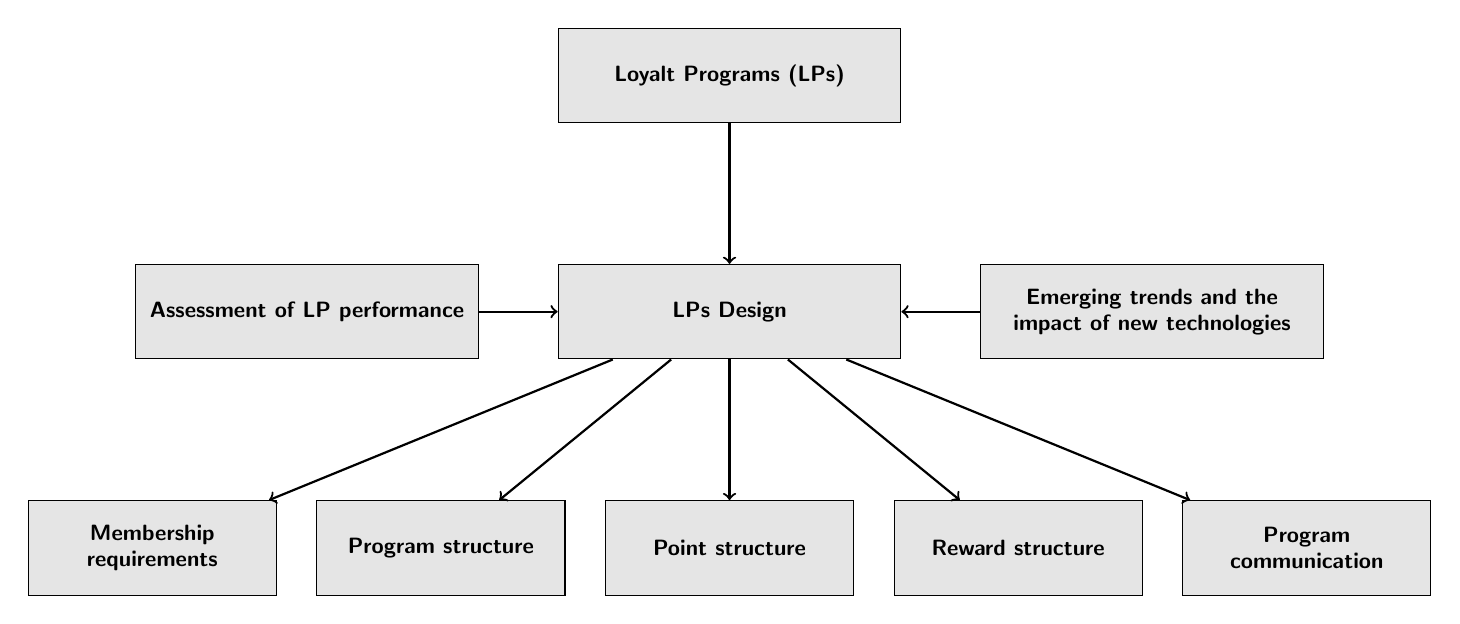
\begin{tikzpicture}
[node distance = 1cm, auto,font=\footnotesize,
% STYLES
every node/.style={node distance=3cm},
% The comment style is used to describe the characteristics of each force
comment/.style={rectangle, inner sep= 5pt, text width=4cm, node distance=0.25cm, font=\scriptsize\sffamily},
% The force style is used to draw the forces' name
force/.style={rectangle, draw, fill=black!10, inner sep=5pt, text width=4cm, text badly centered, minimum height=1.2cm, font=\bfseries\footnotesize\sffamily}] 

% Draw forces
\node [force] (rivalry) {LPs Design};
\node [force, above of=rivalry] (substitutes) {Loyalt Programs (LPs)};
\node [force, left=1cm of rivalry] (suppliers) {Assessment of LP performance};
\node [force, right=1cm of rivalry] (users) {Emerging trends and the impact of new technologies};
\node [force, text width=2.8cm,below of=rivalry] (entrants) {Point structure};
\node [force, text width=2.8cm,left=0.5cm of entrants] (point) {Program structure};
\node [force, text width=2.8cm,right=0.5cm of entrants] (reward) {Reward structure};
\node [force, text width=2.8cm,left=0.5cm of point] (membership) {Membership requirements};
\node [force, text width=2.8cm,right=0.5cm of reward] (communication) {Program communication};
%%%%%%%%%%%%%%%
% Change data from here

% RIVALRY
%\node [comment, below=0.25 of rivalry] (comment-rivalry) {(+) A war against Microsoft\\
%(+) Limiting sunk costs\\
%(+) Coopetition};

% SUPPLIERS
%\node [comment, below=0.25cm of suppliers] {(+) Efficiency\\
%(+) Attracting other developers\\
%(+) Creating a Chrome community};

% SUBSTITUTES
%\node [comment, right=0.25 of substitutes] {(+) Portability};

% USERS
%\node [comment, below=0.25 of users] {(+) Increasing the user information\\
%(+) Reducing the switching costs};

% NEW ENTRANTS


% PUBLIC POLICIES
%\node [comment, text width=3cm, below=0.25 of state] {(+) Positively framed\\
%(+) Transparency\\
%(--) A new monopoly?};

%%%%%%%%%%%%%%%%

% Draw the links between forces
\path[->,thick] 
(substitutes) edge (rivalry)
(suppliers) edge (rivalry)
(users) edge (rivalry)
(rivalry) edge (entrants)
(rivalry) edge (point)
(rivalry) edge (reward)
(rivalry) edge (membership)
(rivalry) edge (communication);

\end{tikzpicture} 
\caption{Literature structure to loyalty programs (based on Breugelmans 2014).}
\label{fig:6forces}
\end{figure}

There are five LPs design components relevant to all types of LPs, (1) membership requirements, (2) program structure, (3) point structure, (4) reward structure, and (5) program communication (Bijmolt et al. 2011; Liu and Yang 2009)\cite{bijmolt2011loyalty}\cite{liu2009competing}.

First of all, membership requirements affect the convenience, effort, and costs associated with joining an LPs (Liu and Yang 2009)\cite{liu2009competing}. The decisions on specific membership requirements involve the trade-offs between attracting a broader customer base by lowering the participation costs and enhancing customer convenience vs. increasing the quality/ profitability of the customer base by being more selective (Breugelmans 2014)\cite{breugelmans2015advancing}. For example, Automatic enrollment in a relation rewards program has positive effects on relational behaviors of self-determined consumers (Dholakia 2006)\cite{dholakia2006customer}. However, we must pay attention to the casual shoppers (cherry pickers) offset subsidies to already loyal customers (Lal and Bell 2003)\cite{lal2003impact}. 

Secondly, there are two predominant program structures: frequency reward programs (FRPs) and customer tiers programs (CTPs) (Blattberg et al., 2008)\cite{blattberg2008byung}. The FRPs take on the form of "buy X amount/collect X points, get a reward", and the CTPs take on the form of "buy X amount/collect X points, qualify for a tier" (Kopalle et al. 2012)\cite{kopalle2012joint}. Which program structrue a company chooses should depend on the industry: FRPs are more common for businesses that hope consumers purchase fruquently and the company are more transaction-focused (e.g., retail business), while CTPs are more common for high commitment, higher price point, and relationship-focused businesse (e.g., airline business).

After that, point structure has been studied extensively in the context of FRPs. For instance, the points-pressure likely encourages customers to increase their purchase frequencies or volume to obtain the reward (Dr`eze and Nunes, 2011; Kivetz et al., 2006; Nunes and Dr`eze, 2006a; Smith and Sparks, 2009a,b)\cite{dreze2008feeling}\cite{kivetz2006goal}\cite{nunes2006endowed}\cite{smith2009s}\cite{smith2009reward}. However, there are more important issues has not been concern, especially in the context of CTPs. Such as, how to determine number of tiers, and how to determine the point issuance ratio (Breugelmans 2014)\cite{breugelmans2015advancing}? Nowdays, the research has become more attractive, the time horizon for redeemable rewards, and the different point earning structures may affect purchase behavior (Breugelmans and Liu 2013)\cite{breugelmans2017effect}.

Furthermore, among the five LP design components, it has been a larger number of studies about reward structure. Frequency reward programs offer rewards that reflect members’ purchase history, through which they have accumulated some form of reward currency (Berman, 2006; Kopalle et al., 2006)\cite{berman2006developing}\cite{kopalle2009dynamic}. This design component includes reward types (monetary vs. nonmonetary), value (luxury vs. necessity) and timing (immediate vs. delayed), actual rewards offered, and their compatibility with the focal brand (Liu and Yang 2009)\cite{liu2009competing}. There are many interesting researches, for example, monetary rewards may reduce customer loyalty, because the rewards may draw attention away from the brand and move it toward the reward itself, which induces spurious loyalty and decreases customers’ intrinsic relationship motivation (Dholakia, 2006; Hennig-Thurau and Paul, 2007; Phillips Melancon et al., 2010; Roehm et al., 2002; Wendlandt and Schrader, 2007)\cite{dholakia2006customer}\cite{hennig2007can}\cite{melancon2011managing}\cite{roehm2002designing}\cite{wendlandt2007consumer}. On the contrary, the non-monetary or soft rewards tend to induce more sustainable loyalty effects because they enhance attitudinal commitment (Phillips Melancon et al., 2010)\cite{melancon2011managing}.

Finally, there has been only limited research on the effectiveness of the different mode of communication in the LPs, but the subtle changes in the way the progress in an LP is communicated could influence consumers' behavior (Wiebenga and Fennis 2014)\cite{wiebenga2014road}.   


How to assess LPs performance, has been a challengeable problem. The main purpose of any LPs is to foster and reward customer loyalty (Bijmolt et al. 2011)\cite{bijmolt2011loyalty}. Customer loyalty consists of two dimension, namely the behavioral decision to repurchase a product over time and the attitudinal attachment to the brand or firm (Dick and Basu, 1994; Uncles et al., 2003)\cite{dick1994customer}\cite{uncles2003customer}. So, how to measure behavioral and attitudinal loyalty is the key. Behavioral loyalty relates to purchase patterns (frequency, volume, and retention), while attitudinal loyalty is expressed in level of commitment, favorable attitudes, positive affect, and so on (Bijmolt et al. 2011)\cite{bijmolt2011loyalty}.

There have been some very tremendous developments in the LP practice in recent years, driven by advancements in information technology, marketing analytics, and consumer interface platforms. Therefore, the LPs of mega-coalitions and mergence of powerful intermediaries are particularly important trends and developments that will shape the evolution of LP management in the future and offer further research opportunities for marketing academics (Breugelmans 2014)\cite{breugelmans2015advancing}. 


\section{Methodology}
\subsection{Model Setup}
Firstly, I prepare to use a 2×2×2 full-factorial, randomized, mixed-effects experimental design. I simplified the reward structure(timing, tyep, value)as described above. Timing of reward redemption (immediate vs. delayed), type of rewards (direct vs. indirect) and value to service experience (satisfied vs. dissatisfied) are designed as between-subject variables (Maxham and Netemeyer 2002)\cite{maxham2002longitudinal}; while two service organization settings (Starbucks and NPO) serve as a within-subject replication factor. The treatment groups are dissimilar from each other by manipulating reward type, reward timing, and service experience through scenario exposures.



Secondly, I prepare to simplify the level of membership (consumers or volunteers) to the following model: A consumer(or volunteer)in the market (or society) chooses whether or not to buy (or participate) a single unit of the product (or once charity activity)from the focal firm (or NPO).

  \begin{table}[ht]
  \centering
    \begin{tabular}{c  c  c }
      \toprule
       $ $ & $\lambda_F$ & $\lambda_I$\\
      \hline
      $V_H$ & HF & HI\\
      \hline
      $V_L$ & LF & LI\\
      \bottomrule
    \end{tabular}
    \caption{The four membership segments}
\end{table}

%Use randomized controlled trials to verify which forms of rewards and points systems are more likely to motivate members (or non-profit volunteers). 









\bibliographystyle{plain}
\bibliography{ref}
\end{spacing}
\end{document}
%%%%%%%%%%%%%%%%%
